\documentclass[landscape,a3paper]{article}

\usepackage{amsmath}
\usepackage{bold-extra}
\usepackage{dirtree}
\usepackage[margin=1.5mm]{geometry}
\usepackage{graphicx}
\usepackage{hyperref}
\usepackage[utf8]{inputenc}
\usepackage{listings}
\usepackage{multicol}
\usepackage{tikz}
\usepackage{xcolor}

\def\cxx{\lstinline[language=C++]}
\def\sh{\lstinline[language=sh]}
\lstset{basicstyle=\ttfamily}
\lstset{
  language=C++,
  defaultdialect=[11]C++,
  tabsize=4,
%  stringstyle=\ttfamily,
  keywordstyle=\color{violet},
  commentstyle=\color{darkgray},
  stringstyle=\color{orange},
  emph={bool,int,unsigned,char,true,false,void}, emphstyle=\color{blue},
  emph={[2]\#include,\#define,\#ifdef,\#endif}, emphstyle={[2]\color{violet}},
  emph={[3]stage}, emphstyle={[3]\color{purple}},
  extendedchars=true,
  escapechar=@,
  mathescape=true,
  escapebegin={\color{darkgray}},
  breaklines=false,
%  frame=lines,
%  backgroundcolor=\color{lightgray},
}

\setlength{\columnsep}{4mm}
\setlength{\columnseprule}{1pt}

\newcommand{\head}[1]{
  \par
  \tikz\node[text width=\linewidth-.6666em,align=justify,fill=lightgray]{#1};
  \par
}

\newcommand{\module}[1]{
  \par
  {%
    \huge\sffamily\bfseries%
    \tikz\node[
      text width=\linewidth-.6666em,
      align=justify,
      fill=black,
      text=white
    ]{\strut#1\strut};%
  }
  \par
}

\setlength\parindent{0pt}

\raggedcolumns

\begin{document}\begin{multicols*}{4}

\module{In General}

\head{\cxx{main()} template}
\begin{lstlisting}
#include <config.h>

#include <dune/common/parallel/mpihelper.hh>

int main(int argc, char **argv)
{
  Dune::MPIHelper::instance(argc, argv);

  // your code goes here
}
\end{lstlisting}

\head{\sh{.cc}-file template}
\begin{lstlisting}
#include <config.h>

// your code and includes go here
\end{lstlisting}

\head{\sh{.hh}-file template}
\begin{lstlisting}
// For a header that is included like
// #include <dune/module/dir/header-name.hh>
#ifndef DUNE_MODULE_DIR_HEADER_NAME_HH
#define DUNE_MODULE_DIR_HEADER_NAME_HH

// your code and includes go here
// do not #include <config.h>

#endif // DUNE_MODULE_DIR_HEADER_NAME_HH
\end{lstlisting}

\module{\cxx{dune-common}}

In the following, \cxx{r} is of type \cxx{R}, which may be a scalar real type,
e.g. \cxx{double} or \cxx{float}.  \cxx{k} is of type \cxx{K}, which may be
may be \cxx{R} or \cxx{std::complex<R>}.

\head{\cxx{template<class K, int size> class FieldVector;}}
\begin{lstlisting}
#include <dune/common/fvector.hh>

FieldVector<K, 2> x = { 0, 1 }; // $x_0:=0, x_1:=1$
FieldVector<K, 2> y(k);         // $x_i:=k\quad\forall i$

assert(i < x.dim()); // get number of entries
k = x[i]; x[i] = k;  // access/assign entry
for(const auto &entry : x)
  k += entry;        // access each entry
for(auto &entry : x)
  entry = k;         // modify each entry

x += y; x -= y; // $x:=x+y$, $x:=x-y$
x *= k; x /= k; // $x:=kx$, $x:=k^{-1}x$
k = x * y;      // $k:=x^Ty=x\cdot y=\sum_i x_iy_i$
k = x.dot(y);   // $k:=x^Hy=\bar x\cdot y=\sum_i\bar x_iy_i$

r = x.one_norm();      // $r:=\sum_i|x_i|$
r = x.two_norm();      // $r:=\smash{\sqrt{\sum_i|x_i|^2}}$
r = x.infinity_norm(); // $r:=\max_i\{|x_i|\}$
\end{lstlisting}
%r = x.two_norm2();     // $r:=\sum_i|x_i|^2$

\head{%
\cxx{template<class K, int rows, int cols>}
\cxx{class FieldMatrix;}
}
\begin{lstlisting}
#include <dune/common/fmatrix.hh>

FieldMatrix<K, 2, 2> S =
{ { 0, 1 },                // $S_{00}:=0,S_{01}:=1$
  { 2, 3 } };              // $S_{10}:=2,S_{11}:=3$
FieldMatrix<K, 2, 2> Q(k); // $Q_{ij}:=k\quad\forall i,j$

assert(i < S.rows()); // get number of rows
assert(j < S.cols()); // get number of columns
k = S[i][j];          // access entry
S[i][j] = k;          // assign entry
for(const auto &row : S)
  for(const auto &entry : row)
    k += entry;       // access each entry
for(auto &row : S)
  for(auto &entry : row)
    entry = k;        // modify each entry

auto L = Q.leftmultiplyany(S);  // $L:=SQ$
auto R = Q.rightmultiplyany(S); // $R:=QS$
Q.leftmultiply(S);              // $S:=SQ$
Q.rightmultiply(S);             // $S:=QS$
S += Q; S -= Q; // $S:=S+Q$, $S:=S-Q$
S.axpy(k, Q);   // $S:=S+kQ$
S *= k; S /= k; // $S:=kS$, $S:=k^{-1}S$
S.invert();     // $S:=S^{-1}$

r = S.frobenius_norm(); // $r:=\smash{\sqrt{\sum_{ij}|S_{ij}|^2}}$
r = S.infinity_norm();  // $r:=\smash{\max_i\{\sum_j|S_{ij}|\}}$
k = S.determinant();    // $k:=\det S$

Q.mv      (x, y); // $y:=Qx$
Q.mtv     (x, y); // $y:=Q^Tx$
Q.umv     (x, y); // $y:=y+Qx$
Q.umtv    (x, y); // $y:=y+Q^Tx$
Q.umhv    (x, y); // $y:=y+Q^Hx$
Q.usmv (k, x, y); // $y:=y+kQx$
Q.usmtv(k, x, y); // $y:=y+kQ^Tx$
Q.usmhv(k, x, y); // $y:=y+kQ^Hx$
Q.solve   (x, y); // find $x$ such that $Qx=y$
\end{lstlisting}

\head{\cxx{#define DUNE_THROW(ExceptionType, message)}}
\begin{lstlisting}
#include <dune/common/exceptions.hh>

if(i > limit)
  DUNE_THROW(Exception, "Error: i > limit ("
             << i << " > " << limit << ")");
\end{lstlisting}

\head{\cxx{template<class T> std::string className();}\\
\cxx{template<class T> std::string className(T& t);}}
\begin{lstlisting}
#include <dune/common/classname.hh>

template<class Vector>
void printTypes(const Vector &v) {
  std::cerr << "Info: Vector type is "
            << className<Vector>()
            << ", entry type is "
            << className(v[0]) << std::endl;
}
\end{lstlisting}

%\cxx{ParameterTree}

%\cxx{DynamicVector<T>} \cxx{DynamicMatrix<T>}
%\cxx{MPIHelper}

\module{\cxx{dune-geometry}}

\head{\cxx{class GeometryType;}}
\begin{lstlisting}
#include <dune/geometry/type.hh>

GeometryType gt;
gt.makeVertex();     gt.makeLine();
gt.makeTriangle();   gt.makeQuadrilateral();
gt.makeTetrahdron(); gt.makePyramid();
gt.makePrism();      gt.makeHexahedron();
gt.makeSimplex(2); // same as makeTriangle()
gt.makeCube(3);    // same as makeHexahedron()
// for each make@\itshape Shape@() there is an is@\itshape Shape@()
assert(gt.isHexahedron());
assert(gt.isCube());   // ignore dimension
assert(gt.dim() == 3); // check dimension
\end{lstlisting}

%\cxx{LocalGeometryTypeIndex} \cxx{GlobalGeometryTypeIndex}

\head{Concept \cxx{Geometry}}
\begin{lstlisting}
using Geo = ...; Geo geo;

using ctype = Geo::ctype;
int ldim = Geo::mydimension;    // local dim
int gdim = Geo::coorddimension; // global dim

Geo::LocalCoordinate  xl; // $\hat x\in\text{ctype}^\text{ldim}$
Geo::GlobalCoordinate x;  // $x\in\text{ctype}^\text{gdim}$
x  = geo.global(xl);      // $x:=g(\hat x)$
xl = geo.local(x);        // $\hat x:=g^{-1}(x)$

// @$J^{-T}\in\text{ctype}^\text{gdim$\times$ldim}$, $J_{ij}:=\partial g_i/\partial\hat x_j$, $\mu:=\sqrt{|\det J^TJ|}$@
Geo::JacobianInverseTransposed JInvT =
  geo.jacobianInverseTransposed(xl);
ctype mu = geo.integrationElement(xl);

GeometryType gt = geo.type(); // shape
assert(i < geo.corners()); // count corners
x = geo.corner(i);         // access corner
x = geo.center();          // @\itshape roughly@
ctype v = geo.volume();    // in global coords
\end{lstlisting}

\head{\cxx{template<class ctype, int dim>}
  \cxx{class ReferenceElements;}}
\begin{lstlisting}
#include <dune/geometry/referenceelements.hh>

using Factory = ReferenceElements<ctype, 3>;
const auto &refTet = Factory::simplex();
const auto &refHex = Factory::cube();
GeometryType gt; gt.makePrism();
const auto &ref = Factory::general(gt);

// Info about ref itself
gt = ref.type();
ctype v = ref.volume();
ref.size(c); // count subentities of codim c

// Info about subentity (i,c)
gt = ref.type(i,c);
// position of barycenter
FieldVector<ctype, 3> x = ref.position(i,c)
// count sub-subentities of codim cc
ref.size(i,c, cc);
// transform number of sub-subentity to ref
ref.subEntity(i,c, ii,cc);
\end{lstlisting}
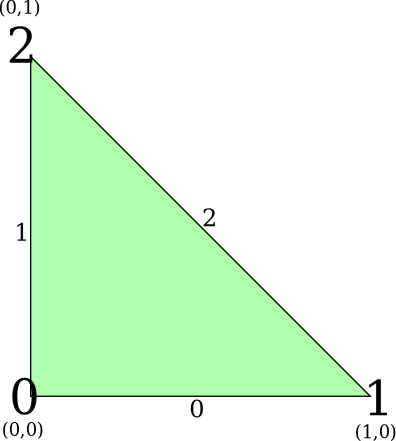
\includegraphics[width=0.5\linewidth]{figures/triangle}
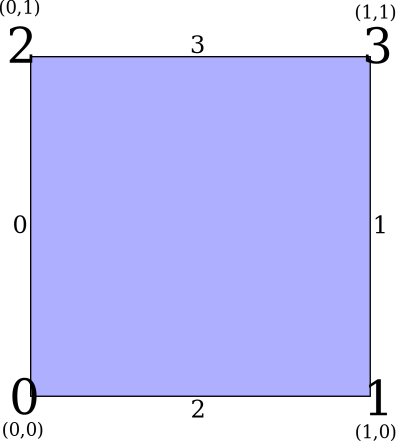
\includegraphics[width=0.5\linewidth]{figures/quadrilateral}
\foreach\shape in {tetrahedron, pyramid, prism, hexahedron} {
  \includegraphics[width=0.5\linewidth]{figures/\shape}
  \includegraphics[width=0.5\linewidth]{figures/\shape_edges}
}

\head{\cxx{template<class ctype, int dim> class QuadratureRules;}}
\begin{lstlisting}
#include <dune/geometry/quadraturerules.hh>

K f(const FieldVector<ctype, dim> &x);
int p; // max polynomial order of f

K result = 0;
GeometryType gt; gt.makeSimplex(dim);
for(const auto &qp :
    QuadratureRules<ctype, dim>::rule(gt, p))
  result += qp.weight() * f(qp.position());
// now result contains the integral of f()
// over the reference-simplex of dimension dim
\end{lstlisting}

TODO: integral over a geometry over a scalar

TODO: integral over a geometry over a gradient (incl piola)

%Virtual refinement

%topologies

\module{\cxx{dune-grid}}

\dirtree{%
.1 \cxx{Grid} (\cxx{YaspGrid}, \cxx{UGGrid}, \cxx{OneDGrid},
   \cxx{GeometryGrid}).
  .2 \cxx{GridView} (\cxx{LevelGridView}, \cxx{LeafGridView}).
    .3 \cxx{IndexSet}.
    .3 \cxx{Entity} (elements, facets, edges, vertices).
      .4 \cxx{Geometry} (entity to global).
    .3 \cxx{Intersection}.
      .4 \cxx{Geometry} (intersection to global).
      .4 \cxx{Entity} (inside/outside element/cell).
      .4 \cxx{Geometry} (intersection to inside/outside).
}

\head{Concept \cxx{Grid} -- hierarchy of meshes}
\begin{lstlisting}
Grid g;

using ctype = Grid::ctype;
int dim  = Grid::dimension;
// think "surface grid"
int dimw = Grid::dimensionworld;

g.globalRefine(); // add a level
assert(g.maxLevel() > 0);
// all coarse/macro entities
auto levelView = g.levelGridView(0);
// all finest/leaf entities
auto leafView = g.leafGridView();
\end{lstlisting}

\head{Concept \cxx{GridView} -- one mesh from the hierarchy}
\begin{lstlisting}
GridView gv;

using Grid = GridView::Grid;
using ctype = GridView::ctype; // as on Grid
int dim  = GridView::dimension;
int dimw = GridView::dimensionworld;

const Grid &g  = gv.grid();
const auto &is = gv.indexSet();
// count entities...
int n = gv.size(c);  // with codim c
int n = gv.size(gt); // with GeometryType gt

// iterate over entities in gv
for(const auto &elem   : elements(gv)) ...;
for(const auto &facet  : facets  (gv)) ...;
for(const auto &edge   : edges   (gv)) ...;
for(const auto &vertex : vertices(gv)) ...;
// iterate intersections of elem in gv
for(const auto &isect  :
      intersections(gv, elem)) ...;
\end{lstlisting}

\head{Concept \cxx{IndexSet} -- numbering within \cxx{GridView}s}
Entities of different shape (\cxx{GeometryType}) are numbered separately.
% -- a triangular entity may have the same index as a quadrilateral entity
% within the same grid view.
See \cxx{MultipleCodimMultipleGeomTypeMapper}.
\begin{lstlisting}
const IndexSet &is;

Entity e; // any codim
int i, c; // number/codim of subentity
is.index(e);         // index of e in gv
is.subIndex(e, i,c); // index of subentity
\end{lstlisting}

\head{Concept \cxx{Entity<codim>} -- elements, facets, edges, vertices}
\begin{lstlisting}
Entity e;

// all entities: mydim + codim == dim
// elements: codim == 0; facets:   codim == 1
// edges:    mydim == 1; vertices: mydim == 0
int codim = Entity::codimension;
int dim   = Entity::dimension; // as on Grid
int mydim = Entity::mydimension;

GeometryType gt = e.type(); // Shape
// the LevelGridView that e is part of
int l = e.level();

// transform mydimension -> dimensionworld
Entity::Geometry geo = e.geometry();
\end{lstlisting}

\head{Concept \cxx{Intersection} -- connectivity between elements}
\begin{lstlisting}
Intersection is;

using ctype = Intersection::ctype;
// local coords  (== Grid::dimension - 1)
int mydim = Intersection::mydimension;
// global coords (== Grid::dimensionworld)
int dimw  = Intersection::dimensionworld;

GeometryType gt = is.type(); // Shape

// transform intersection -> world
Intersection::Geometry geo = is.geometry();
Intersection::LocalCoordinate  xl;
Intersection::GlobalCoordinate nu_u, nu_q;
// $\|\nu_u\|_2=1$, $\nu_q:=\nu_u\cdot\text{geo.integrationElement(xl)}$
nu_u = is.unitOuterNormal(xl);
nu_q = is.integrationOuterNormal(xl);

using Element = Intersection::Entity;
using LGeo    = Intersection::LocalGeometry;

// inside element (always exists)
Element in  = is.inside();
// transform intersection -> inside
LGeo inGeo  = is.geometryInInside();
// index of sub-facet of in that contains is
int inIdx   = is.indexInInside();

if(is.neighbor()) { // check outside exists
  Element out = is.outside();
  LGeo outGeo = is.geometryInOutside();
  int outIdx  = is.indexInOutside();
} // otherwise on domain boundary
\end{lstlisting}

%mapper: mcmg, scsg, universal

\head{\cxx{template<int dim> class YaspGrid;}\\
  Yet Another Structured Parallel Grid}
Implements concept \cxx{Grid}.
\begin{lstlisting}
#include <dune/grid/yaspgrid.hh>

// construct unit square $[0,1]^2$ with one element
YaspGrid<2> grid0({ 1, 1 }, { 1, 1 });

// construct cube $[-1,1]^3$ with $8=2^3$ elements
YaspGrid<3> grid1({ -1, -1, -1 }, { 1, 1, 1 },
                  { 2, 2, 2 });
\end{lstlisting}
%\cxx{GeometryGrid} \cxx{OneDGrid} \cxx{UGGrid}

%Input: \cxx{GmshReader} \cxx{StructuredGridFactory}

\head{\cxx{template<class GridView> class VTKWriter;}\\
  Generate files for \sh{paraview}}
\begin{lstlisting}
#include <dune/grid/io/file/vtk/vtkwriter.hh>

GridView gv;
double f(FieldVector<ctype, dim> xg);

// for multiple possible GeometryTypes use
// MultipleCodimMultipleGeomTypeMapper instead
const auto &is = gv.indexSet();

// interpolate f to piecewise constants
std::vector<double> p0(gv.size(0))
for(const auto &e : elements(gv))
  p0[is.index(e)] = f(e.geometry().center());

// interpolate f to P1/Q1
std::vector<double> p1(gv.size(dim));
for(const auto &v : vertices(gv))
  p1[is.index(v)] = f(v.geometry().center());

// output the two interpolations of f
VTKWriter<GridView> writer(gv);
writer.addCellData(p0, "constants");
writer.addVertexData(p1, "linears");
writer.write("file_name_base");
\end{lstlisting}

%Output: \cxx{SubSamplingVTKWriter} gnuplot

\module{\cxx{dune-istl}}

\cxx{BlockVector} \cxx{BCRSMatrix}

\cxx{MatrixAdapter} \cxx{Preconditioner}

list of preconditioners

\cxx{Solver} Interface \cxx{InverseOperatorResult}

list of solvers

\module{\cxx{dune-localfunctions}}

local finite element interface -> { local basis interface, local interpolation
  interface, local coefficients interface }

list of local finite elements


\end{multicols*}\end{document}


% tell emacs to use pdflatex
%%% Local Variables:
%%% mode: latex
%%% mode: TeX-PDF
%%% TeX-master: t
%%% mode: flyspell
%%% ispell-local-dictionary: "en_US"
%%% End:
